\documentclass{svproc}
\usepackage{url}
\usepackage{graphicx}
\usepackage{adjustbox}
\usepackage{float}
\def\UrlFont{\rmfamily}

\begin{document}
\mainmatter
\title{Comparative Study of Artificial Intelligence algorithms for Othello
}
\subtitle{CS7IS2 Project (2019/2020)}
\author{Esmond D'Souza, Hemlata M Sharma, Oommen Kuruvilla, \and Tejas Munees}
\authorrunning{E. D'Souza, H. Sharma, O. Kuruvilla \and T. Munees}

\institute{
\email{dsouzae@tcd.ie, sharmah@tcd.ie, kuruvilo@tcd.ie, sivaramt@tcd.ie}}

\maketitle              % typeset the title of the contribution

\begin{abstract}
This paper studies and analyses different artificial intelligence algorithms and their performance, by implementation on the game, Othello. Othello is a two-player, zero sum and perfect information game. This study uses 3 different algorithms, namely, Minimax, Expectimax, and Alpha-Beta Pruning, along with a random agent. We make the agents play against each other with different difficulty settings, determined by the depth of the search and record wins, scores, and average time per move by both agents in every game. These are then compared in an exploratory nature.

\keywords{Othello, Artificial Intelligence, minimax, expectimax, alpha-beta pruning, agents, tree-search}
\end{abstract}
%

\section{Introduction}

Artificial Intelligence (AI) is major part of computer games and the role they play has only continued to increase as time progress as a reason of complex game-play, environment and in-game interactive objects. While the research interest in artificial intelligence is in its peak today, the implementation of it, and an attempt to use that in games is nothing new. This is an area that dates back to 1960s.

Around 1968, a chess master named David Levy challenged John McCarthy, who is known as the founder father of AI, that no computer would beat the a grand master within ten years. After five years of John had given up only because it had become certain that computers won't be able to play or win the way humans did \cite{MIT_lecture}.

20 odd years later, IBM's Deep Blue beat the world chess champion with two wins, one lost and three draws. Although McCarty could've been right on computers not playing the way humans did, today we have one of the closest representation to human's way of playing- neural networks. Deep Chess is one such network created by Omid E. David, Nathan S. Netanyahu and Lior Wolf \cite{deepchess} which uses several layers of neural networks in its model.

However long before our portable computers became powerful and sophisticated enough to run deep neural networks, we had complex artificial intelligence models like Deep Blue. Most of such models use a brute-force search approach, albeit they did them intelligently.

While it is easy to neglect a brute force search algorithm as not an intelligent solution. But it is important to understand the intelligence factor in such searching. In chess for example, in order to brute force search one move followed by potential opponents and self's moves till the end of the tree, it would easily reach the order of 10\textsuperscript{120} and to put that in perspective, the number of nanoseconds in the entire history of universe is of the order 10\textsuperscript{106} \cite{MIT_lecture}. Hence the computation becomes impossible and therefore the intelligence component becomes vital in such models, and even so when it is required to be competent enough to beat the world champion. In this paper, we discuss such artificial intelligence and implement them for the game Othello. We try to compare the number of wins, scores, and average time per move.

\subsection{Othello}

Othello also known as Reversi, like chess and checkers is a two-player game. According to game theory, Othello is deterministic, zero sum and perfect information game. The game is deterministic is because any move done by the player has no degree of randomness to where it could land. The probability of the move going to the position where the player intended it to go is 100\%. The game is zero sum because of its nature where of you add the gains of both player and subtract it with their loses, the sum becomes zero. Here the gain is the number of player's own pieces and loses is given by the number of opponent's pieces and because of this, the game is adversarial in nature. Also, the game is a perfect information game as it a sequential-move based game, where a player is able to see what the other player has done before choosing their own next move and also a player is capable of knowing their opponent's possible moves. The goal of the game is to have the maximum number of disks of the two players to win.

\begin{figure}
\centering
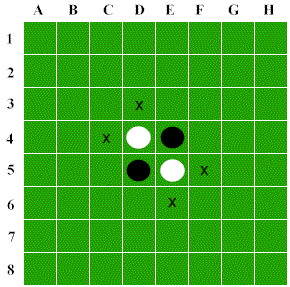
\includegraphics[scale=0.5]{img1.png}
\caption{Initial State of the board. (Taken from \cite{image_website})} \label{fig1}
\end{figure}

The game begins in a state as shown in Figure \ref{fig1}, where the white and black pieces are placed at D4, E5 and E4, D5 respectively. The black piece always begins the game where the initial valid/legal moves for the black are given by ‘x’ in Figure \ref{fig1}. A move is considered valid or legal only if a player (lets say, Player\_1) is able to land a piece on board where there is at least one opponent piece in between the position where the Player\_1 is about to place the piece and a another piece that has already been previously landed on board by the Player\_1. This is allowed horizontally, vertically and diagonally and combinations of these as well. Once Player\_1 has made such a valid move, the opponent's pieces in between are flipped to the opposite color and becomes Player\_1's pieces. The game generally ends when both players are unable to make anymore valid or legal moves. While there exists smaller version of the board, it is generally played in an 8x8 board and we would use the same in this paper.

The paper is organised as follows: Section \ref{2} discusses the state of the art in artificial intelligence specially their implementation in the game Othello. Section \ref{3} talks about the algorithms used in this research and its results in Section \ref{4}. The paper then is concluded in Section \ref{5}.

\section{Related Work}\label{2}

As mentioned earlier, techniques like neural networks, reinforcement learning, and ensemble models amongst many others have today become possible because of high computational resources. These techniques and many other new ones are the state of the art techniques used for games like Othello.

One such research was conducted by authors Skoulakis, I.E. and Lagoudakis in 2012 \cite{esmond_1}. The authors suggest a novel technique of using reinforcement learning efficiently for adversarial games. Sequential-move based games often need decision making concerning the moves. Artificial intelligence search algorithms like min-max and its modifications often help in the same by using Temporal Difference (TD) learning that strives on bootstrapping methods to evaluate how optimal a move is \cite{esmond_1}.

These evaluation functions paired up with temporal differences commonly face issues as historical game data is not taken into consideration and the evaluation function is just updated incrementally based on the current actions. As the computer can't process all the future steps and limits it to a considerable depth value, this results in the computer learning to make the best decision in the current context only not considering all the possible moves as mentioned earlier.

The authors propose a novel algorithm under the name, Least-Squares Policy Iteration (LSPI). This algorithm updates the evaluation function based on the current and passed state, the reward received per action, the rewards received in the past games played by the computer or even games played by other agents. As a result, at each step of interaction, the computer observes the current state, selects the calculated action to be taken, and observes the resulting next state along with the reward received \cite{esmond_1}.

The main change in the LSPI algorithm to make it suitable for the adversarial game environments is the calculation of the evaluation policy in the result for the next state. The authors accomplished this by using a shallow minimax searching algorithm to get the best response of Min and Max. As compared to the traditional TD learning method, this algorithm makes batch updates to the evaluation function without bootstrapping with the collection of samples from previous games, or old samples even played by other agents \cite{esmond_1}.

As for the evaluation part the authors used and compared three different types of models to assess the benefits and drawbacks of the LSPI algorithm during adversarial gaming. For this experiment, the models used were the TD (Self-play), LSPI (TD Samples) and LSPI (Self-play) models. The TD (Self-play) model learns from itself in the current context using its passed moves and the moves of the opponent as samples, which is the considered the typical way for adversarial games \cite{esmond_1}. The LSPI (TD Samples) models use the LSPI algorithm along with the TD Samples only to check the efficiency of both given the same sample space, and finally, the LSPI (Self-play) model learns from its current game playing moves, along with its opponents moves, its moves of games played against other agents and games played by other agents.

The result clearly states that the LSPI (Self-playing) models perform the best with less number of samples, however, the learning curve flattens after a while as the same agents play with the same moves continuously. On the contrary, the LSPI (TD-samples) model benefits from the variability of the TD learning algorithm and has a steady learning curve right from the start which in time constantly improves, however it performs low as compared to the first model with the same number of samples. The authors of this paper conclude by comparing the improvement of the LSPI learning method over the traditional TD learning \cite{esmond_1}.

A similar state of the art by authors, K. Kim, H. Choi and S. Cho examines an ensemble/hybrid model of evolution and reinforcement learning for Othello in their research work \cite{esmond_2}. They suggest the combination of the evaluation algorithm along with reinforcement learning to boost the capabilities of the agent playing the game.

The top Othello programs like \emph{Lositello}, \emph{Ntest} and \emph{Xzebra} have their pre-evaluated calculations for the moves in the initial stage and then the evaluation functions update depending on the gameplay. The authors suggest the combination of the evaluation algorithm with temporal learning at the beginning of the game as an opening book rule and then incrementally update and discover more knowledge using reinforcement learning \cite{esmond_2}. The latter is done by using the rules from self-playing and endgame solver that computes the stage at the end of the game.

This method according to the authors consists of two parts, first with the help of temporal learning, premature solutions are identified which correspond to the high-performance actions. After this, the evolutionary algorithm is used to further filter down and find better actions to be taken. The population of the evolutionary algorithm could be initialised by leveraging the previous knowledge from self-playing. To perform efficiently, the evolutionary algorithm can utilise the previously discovered knowledge from the reinforcement learning. This, in turn, would help them discover better strategies.

The initial moves could either be decided from drawing all good and bad moves with the help of subject matter experts or access the scores of each move by comparing the results of the previous games with those moves \cite{esmond_2}. The authors have also made use of neural networks for evaluation of the board configuration, and for all the other steps, reinforcement learning using the opening choices and/or endgame knowledge was evaluated. For the model evaluation, the authors compared and contrasted four models namely \cite{esmond_2},

\begin{enumerate}
\item EV - evolution model with no knowledge
\item EV\_O - evolution model with opening knowledge
\item EV\_E - evolution model with endgame knowledge
\item EV\_O\_E - evolution model with opening and endgame knowledge.
\end{enumerate}

The main point highlighted here by the authors was the performance gain of the EV\_E model over the EV\_O model in the majority of the cases \cite{esmond_2}. EV\_E performed considerably low in the early stages but reversed the results at the end of the game. The authors conclude the benefits of using domain knowledge while playing Othello and prove the benefits of using both types of knowledge (opening and endgame) was highly beneficial as compared to either one \cite{esmond_2}.

However optimisation need not necessarily come by trying out different from algorithms, forming gaming strategies for any game AI model is also equally essential, which is explained by authors C. Frankland and N. Pillay in \cite{hema_1}.This study explains how Genetic Programming is used to optimise game playing for an Othello player.

Genetic Programming (GP) encodes Darwin’s ‘Survival of the fittest’ theory. In GP, members of the population are represented by solution trees and evaluation of the fittest is done using heuristics. Throughout the game, the player does not stick to one solution tree, instead a combination of the best tree is used for every move.

In this study, the initial population is randomly generated and each heuristic represented as an area of the board. Each square falls into a particular category. For example, the four corners are in the corner defence category and have the same heuristic value. In addition to the board heuristics, there exists boolean strategy heuristics. For example, the ‘tCnrH’ heuristic when set \emph{TRUE}, gives priority to corner points and doubles the heuristic value at a corner point \cite{hema_1}.

In this strategy, the first element of the population plays against the alpha player a number of times. An alpha player can be randomly generated at the start or be carried forward from the previous game. The fitness of an element is calculated by the number of wins and ties. A win is rewarded with two points while a tie is rewarded by one point. The winner becomes an alpha player and competes with the next element of the population and so on, until all elements of the population have played against the alpha. Tournament Selection is used to choose the parents of the next generation.

Since GP is a machine learning approach, the performance is better than traditional search algorithms. However according to the authors, an initial population size of greater than 100 can significantly reduce the speed of computation \cite{hema_1}.

All the state of the art studies discussed above present a novel and interesting implementation of different strategies. As a way forward to such implementations, in this study we would implement a basic AI agent game strategies and build the game with rules and regulations, which would enable us in future to build novel and state of the art strategies for the game, Othello.

\section{Algorithms}\label{3}

In this project, we have implemented four different strategies with depth variations to few of them. They are,

\begin{itemize}
    \item Random
    \item Minimax
    \item Alpha-Beta Pruning
    \item Expectimax
\end{itemize}

The input to all these algorithms is a list of legal moves for the agent, the current board positions and other parameters that are required based on the algorithms, when it is the agent’s turn to play. The list of legal moves is a list of positions where the agent can place a disk such that one or more of the opponent’s disks get flipped. For the random strategy, the agent randomly selects a move from the list of legal moves. For the remaining of the algorithms, Search trees are generated to a limited depth, chosen based on difficulty levels, Easy, Medium and Hard having depths 3, 5, and 7 respectively. A  search tree is expanded by each of the legal moves. Moves on the first level are legal moves for the agent, the nodes on the next level are legal moves for the opponent player/agent for each of the nodes on the first level. At the leaf nodes on the bottom of the tree, heuristics is calculated as the total number of disks of the agent/player based on the weighted score.

In minimax, for each level of agent's moves, the agent picks the move that will maximize its utility assuming that the opponent player chooses a move that minimizes the agent’s utility. All possible nodes are explored in order to choose the best move.
Alpha-beta pruning is a more efficient version of the minimax algorithm where not all nodes are explored. Iterative Deepening Depth-First Search (IDDFS) is used. The record of the best possible utility for maximizers and minimizers is maintained.  The values are updated only if a maximizer encounters a higher utility node and if a minimizer encounters a lower utility node. Higher utility nodes have no effect on the value of the minimizer and lower utility nodes have no effect on the value of the minimizer. This way a good number of branches are pruned, saving computational cost and time.

Expectimax is similar to minimax, except, instead of minimisers, we have chance nodes. These chance nodes helps the algorithm to take risk that either allows for a higher utility state or a lower utility state. These chance nodes are expected (mean) values of their children nodes. This makes expectimax as not 100\% safe, as there is a possibility of a lower utility state. As depth increases, probability of reaching a given search node decreases making it more damaging. Since there is no pruning possible for expectimax, it can become very slow, depending on the unexplored children.

We also used Score board Heuristic as seen in Table \ref{board} which was derived from \cite{hboard}. This heuristic is used to calculate score internally which the algorithms try to maximise and minimise as necessary where each box corresponds to a similar position on the game board.

\begin{table}[H]
\centering
\begin{adjustbox}{width=4cm,center}
\resizebox{\textwidth}{!}{%
\begin{tabular}{|l|l|l|l|l|l|l|l|}
\hline
120 & -20 & 20 & 5  & 5  & 20 & -20 & 120 \\ \hline
-20 & -40 & -5 & -5 & -5 & -5 & -40 & -20 \\ \hline
20  & -5  & 15 & 3  & 3  & 15 & -5  & 20  \\ \hline
5   & -5  & 3  & 3  & 3  & 3  & -5  & 5   \\ \hline
5   & -5  & 3  & 3  & 3  & 3  & -5  & 5   \\ \hline
20  & -5  & 15 & 3  & 3  & 15 & -5  & 20  \\ \hline
-20 & -40 & -5 & -5 & -5 & -5 & -40 & -20 \\ \hline
120 & -20 & 20 & 5  & 5  & 20 & -20 & 120 \\ \hline
\end{tabular}%
}
\end{adjustbox}
\caption{Score Board Heuristic}
\label{board}
\end{table}

\section{Experimental Results}\label{4}

Our strategies are represented as agents in our project. To evaluate the performance of our agents/players, we tested them against each other in such a way that every agent played six games against every other agent, three of which were started with one agent playing first, with all possible difficulty settings.

Minimax , Alpha-beta and Expectimax have three potential agents each, one for each difficulty level: easy, medium and hard, while random has only one potential agent. For each game between two agents, we took into the count of wins, account score of each agent, avg time taken by an agent for a move.

Table \ref{table1} shows us the total wins by each agent with various difficulty level over a set of three games. We can also see the percentage of total score gained and lost across rows and columns respectively in over three games by each agent over the same set of three games in Table \ref{table2}. In both Table \ref{table1} and Table \ref{table2}, $\alpha\beta$ stands for \emph{Alpha-Beta} Agent  $MM$ stands for \emph{Minimax} Agent and $EM$ stands for \emph{Expectimax} Agent and numbers 3, 5 and 7, specifies the depth of the search used, by setting the difficulty to Easy, Medium and Hard respectively. Each game started with a unique first move, to make sure that the data was not redundant and results not skewed.


\begin{table}[H]
\centering
\resizebox{\textwidth}{!}{%
\begin{tabular}{|l|l|l|l|l|l|l|l|l|l|l|l|}
\hline
\textbf{Algorithm}    & \textbf{Random} & \textbf{$\alpha\beta$-3} & \textbf{$\alpha\beta$-5} & \textbf{$\alpha\beta$-7} & \textbf{MM-3} & \textbf{MM-5} & \textbf{MM-7} & \textbf{EM-3} & \textbf{EM-5} & \textbf{EM-7} & \textbf{$\Sigma$ Wins} \\ \hline
\textbf{Random}       & -               & 0                     & 0                     & 0                     & 0                  & 0                  & 0                  & 3                     & 2                     & 3                     & 8                    \\ \hline
\textbf{$\alpha\beta$-3} & 3               & -                     & 0                     & 0                     & 3                  & 1                  & 2                  & 1                     & 1                     & 3                     & 14                   \\ \hline
\textbf{$\alpha\beta$-5} & 3               & 3                     & -                     & 1                     & 3                  & 3                  & 1                  & 3                     & 1                     & 2                     & 20                   \\ \hline
\textbf{$\alpha\beta$-7} & 3               & 3                     & 3                     & -                     & 3                  & 3                  & 2                  & 3                     & 3                     & 3                     & 26                   \\ \hline
\textbf{MM-3}    & 2               & 0                     & 0                     & 0                     & -                  & 1                  & 0                  & 3                     & 2                     & 3                     & 11                   \\ \hline
\textbf{MM-5}    & 3               & 1                     & 0                     & 1                     & 2                  & -                  & 2                  & 3                     & 3                     & 3                     & 18                   \\ \hline
\textbf{MM-7}    & 3               & 1                     & 1                     & 0                     & 3                  & 3                  & -                  & 3                     & 3                     & 3                     & 20                   \\ \hline
\textbf{EM-3} & 0               & 0                     & 0                     & 0                     & 0                  & 0                  & 0                  & -                     & 1                     & 2                     & 3                    \\ \hline
\textbf{EM-5} & 1               & 0                     & 1                     & 0                     & 1                  & 0                  & 0                  & 3                     & -                     & 1                     & 7                    \\ \hline
\textbf{EM-7} & 3               & 1                     & 0                     & 0                     & 0                  & 0                  & 0                  & 3                     & 3                     & -                     & 10                   \\ \hline
\end{tabular}%
}
\caption{Total wins by different agents over three games}
\label{table1}
\end{table}

\begin{table}[H]
\centering
\resizebox{\textwidth}{!}{%
\begin{tabular}{|l|l|l|l|l|l|l|l|l|l|l|}
\hline
\textbf{Algorithm}    & \textbf{Random} & \textbf{$\alpha\beta$-3} & \textbf{$\alpha\beta$-5} & \textbf{$\alpha\beta$-7} & \textbf{MM-3} & \textbf{MM-5} & \textbf{MM-7} & \textbf{EM-3} & \textbf{EM-5} & \textbf{EM-7} \\ \hline
\textbf{Random}       & -               & 34.9\%                & 31.94\%               & 34.38\%               & 25.0\%             & 30.21\%            & 19.25\%            & 68.75\%               & 47.92\%               & 63.02\%               \\ \hline
\textbf{$\alpha\beta$-3} & 65.63\%         & -                     & 41.15\%               & 44.79\%               & 65.63\%            & 35.42\%            & 57.29\%            & 43.75\%               & 41.61\%               & 71.35\%               \\ \hline
\textbf{$\alpha\beta$-5} & 64.06\%         & 59.9\%                & -                     & 43.75\%               & 60.94\%            & 56.02\%            & 50.0\%             & 67.19\%               & 53.13\%               & 52.6\%                \\ \hline
\textbf{$\alpha\beta$-7} & 59.9\%          & 73.58\%               & 69.79\%               & -                     & 68.23\%            & 70.31\%            & 60.94\%            & 100.0\%               & 100.0\%               & 66.15\%               \\ \hline
\textbf{MM-3}    & 45.31\%         & 37.44\%               & 27.6\%                & 26.04\%               & -                  & 42.19\%            & 0.0\%              & 71.35\%               & 68.64\%               & 79.57\%               \\ \hline
\textbf{MM-5}    & 70.17\%         & 41.15\%               & 40.1\%                & 38.54\%               & 50.0\%             & -                  & 59.9\%             & 84.43\%               & 93.29\%               & 79.58\%               \\ \hline
\textbf{MM-7}    & 86.87\%         & 40.1\%                & 45.31\%               & 34.38\%               & 86.98\%            & 66.3\%             & -                  & 97.95\%               & 100.0\%               & 96.27\%               \\ \hline
\textbf{EM-3} & 30.57\%         & 44.79\%               & 33.85\%               & 24.48\%               & 5.17\%             & 30.21\%            & 31.58\%            & -                     & 52.6\%                & 49.48\%               \\ \hline
\textbf{EM-5} & 26.56\%         & 41.67\%               & 45.31\%               & 32.81\%               & 40.1\%             & 20.45\%            & 5.06\%             & 72.92\%               & -                     & 55.21\%               \\ \hline
\textbf{EM-7} & 36.98\%         & 41.67\%               & 43.23\%               & 35.94\%               & 29.17\%            & 13.58\%            & 0.0\%              & 51.83\%               & 55.21\%               & -                     \\ \hline
\end{tabular}%
}

\caption{Percentage of Total Scores achieved and lost across Agents}
\label{table2}
\end{table}

From Table \ref{table1} and Table \ref{table2}, we could deduce that the best performing algorithm was Alpha-Beta with depth 7, by sheer count of total number of wins, followed by Minimax. While Alpha-Beta, is just a variant of minimax including pruning, the wins could be determined by the start move. One of the worst performers was expectimax. The reason, as mentioned in Section \ref{3}, is that unlike minimax, Expectimax has chance nodes, which generally takes risks, and could end up at a lower utility state, which has happened in our experimentation as well. Although, there are few wins as well, which also proves that such risks taken by chance nodes, also sometimes lead up to a higher utility state.

We also see the stacked-bar plot in Figure \ref{2}, comparing the log of time taken for each algorithm to make a move when played with other algorithms. We can see that \emph{Expectimax} with depth 7 took the highest time to finish the game. This is given by the Expectimax algorithm's inability to prune, thus making it slow. On the other hand, we were can see the benefits of pruning in Alpha-Beta algorithm. With depth 7, we see the Alpha-Beta is faster than Expectimax's depth 5. Random agent performed the fastest as seen in Figure \ref{2} because of lack of time-intensive tasks such as tree-search.

\begin{figure}
    \centering
    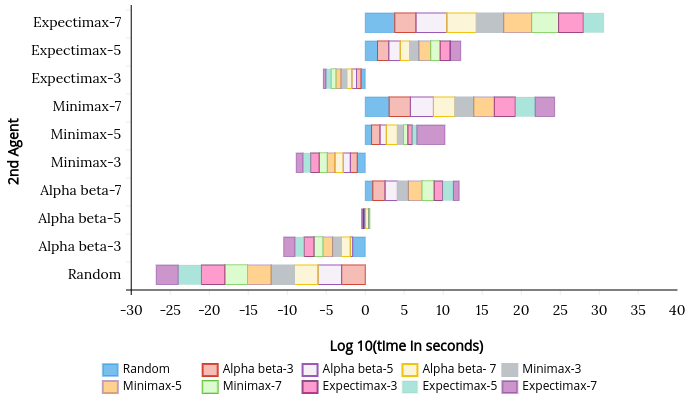
\includegraphics[scale=0.49]{img2.png}
    \caption{Log of Time taken per move across different first agent, by the second agent}
    \label{figure2}
\end{figure}

\section{Conclusion}\label{5}

In this study, the evaluation of two-player game, Othello by different AI agents/ algorithms was investigated. We discussed the AI's role in computer games and how, while they have changed over the recent years, the implementation of intelligent search approach still continues to perform very well in board games like chess, checkers, and Othello amongst others. We also discussed the state-of-the-art solutions for Othello, how a “search-AI agent” implementation, as done in this study, could set up the foundation for such novel ideas.
While the study has been performed for several experiments, over long duration, the authors still felt that the number of games could be vastly increased than three. This, however was because of limitations in accessing powerful hardware.

Games like Othello which are perfect information, deterministic, and zero sum, leaves algorithm like expectimax with chance nodes, weak. Even more so, against players like Alpha-Beta or minimax with depth 7. As the probability of taking risk becomes high over several moves and yet still Alpha-Beta/minimax can make a best possible move for that current game state. The authors also feel that expectiminimax could be compared along with expectimax in future works.

The authors would like to mention the study has given an in-depth insight into how two-player games are made and how parameters like depth influences the difficulty level in a game. The study has also given us the importance of balancing performance for processing time, as in a computer game, humans would not necessarily wait for longer periods for computer to make a move.

We also would like to continue our work on this in future, with more experiments, different strategies including few state-of-the-art, utilising time and resources as necessary.


\begin{thebibliography}{6}
%

\bibitem{MIT_lecture}
Patrick Winston.  6.034. Artificial Intelligence. Fall 2010. Massachusetts Institute of Technology: MIT OpenCourseWare, \url{https://ocw.mit.edu/}. License: Creative Commons BY-NC-SA.

\bibitem{deepchess}
David, Omid E., Nathan S. Netanyahu, and Lior Wolf. “DeepChess: End-to-End Deep Neural Network for Automatic Learning in Chess.” Lecture Notes in Computer Science (2016): 88–96. Crossref. Web.

\bibitem{image_website}
“Games for Young- Othello” webpage,
\url{https://www.gamesforyoungminds.com/blog/2018/3/23/othello-review}.
Last Accessed on 30 March 2020.

\bibitem{esmond_1}
Skoulakis, Ioannis E. and Michail G. Lagoudakis. “Efficient Reinforcement Learning in Adversarial Games.” 2012 IEEE 24th International Conference on Tools with Artificial Intelligence 1 (2012): 704-711.

\bibitem{esmond_2}
K. Kim, H. Choi and S. Cho, "Hybrid of Evolution and Reinforcement Learning for Othello Players," 2007 IEEE Symposium on Computational Intelligence and Games, Honolulu, HI, 2007, pp. 203-209.

\bibitem{hema_1}
C. Frankland and N. Pillay, "Evolving game playing strategies for Othello," 2015 IEEE Congress on Evolutionary Computation (CEC), Sendai, 2015, pp. 1498-1504.

\bibitem{hboard}
T. S. Somasundaram, K. Panneerselvam, T. Bhuthapuri, H. Mahadevan and A. Jose, "Double Q–learning Agent for Othello Board Game," 2018 Tenth International Conference on Advanced Computing (ICoAC), Chennai, India, 2018, pp. 216-223.

\end{thebibliography}
\end{document}
